\subsection*{Plagiatsklausel}

Hiermit versichern wir, dass wir diese Projektarbeit selbständig verfasst und keine
anderen als die angegebenen Quellen und Hilfsmittel benutzt haben. Die Stellen
unserer Arbeit, die dem Wortlaut oder dem Sinn nach anderen Werken entnommen
sind, haben wir in jedem Fall unter Angabe der Quelle als Entlehnung kenntlich
gemacht. Dasselbe gilt sinngemäß für Tabellen, Karten und Abbildungen. Diese Arbeit
hat in dieser oder einer ähnlichen Form noch nicht im Rahmen einer anderen Prüfung
vorgelegen.

\begin{figure}[hbtp]
	\centering
	
\includegraphics[width=.5\linewidth, page=1]{reference/signature/l_sign.png}
	\caption{Signature}
\end{figure}

\pagebreak

\subsection*{Class Diagram}

\begin{figure}[hbtp]
	\centering
	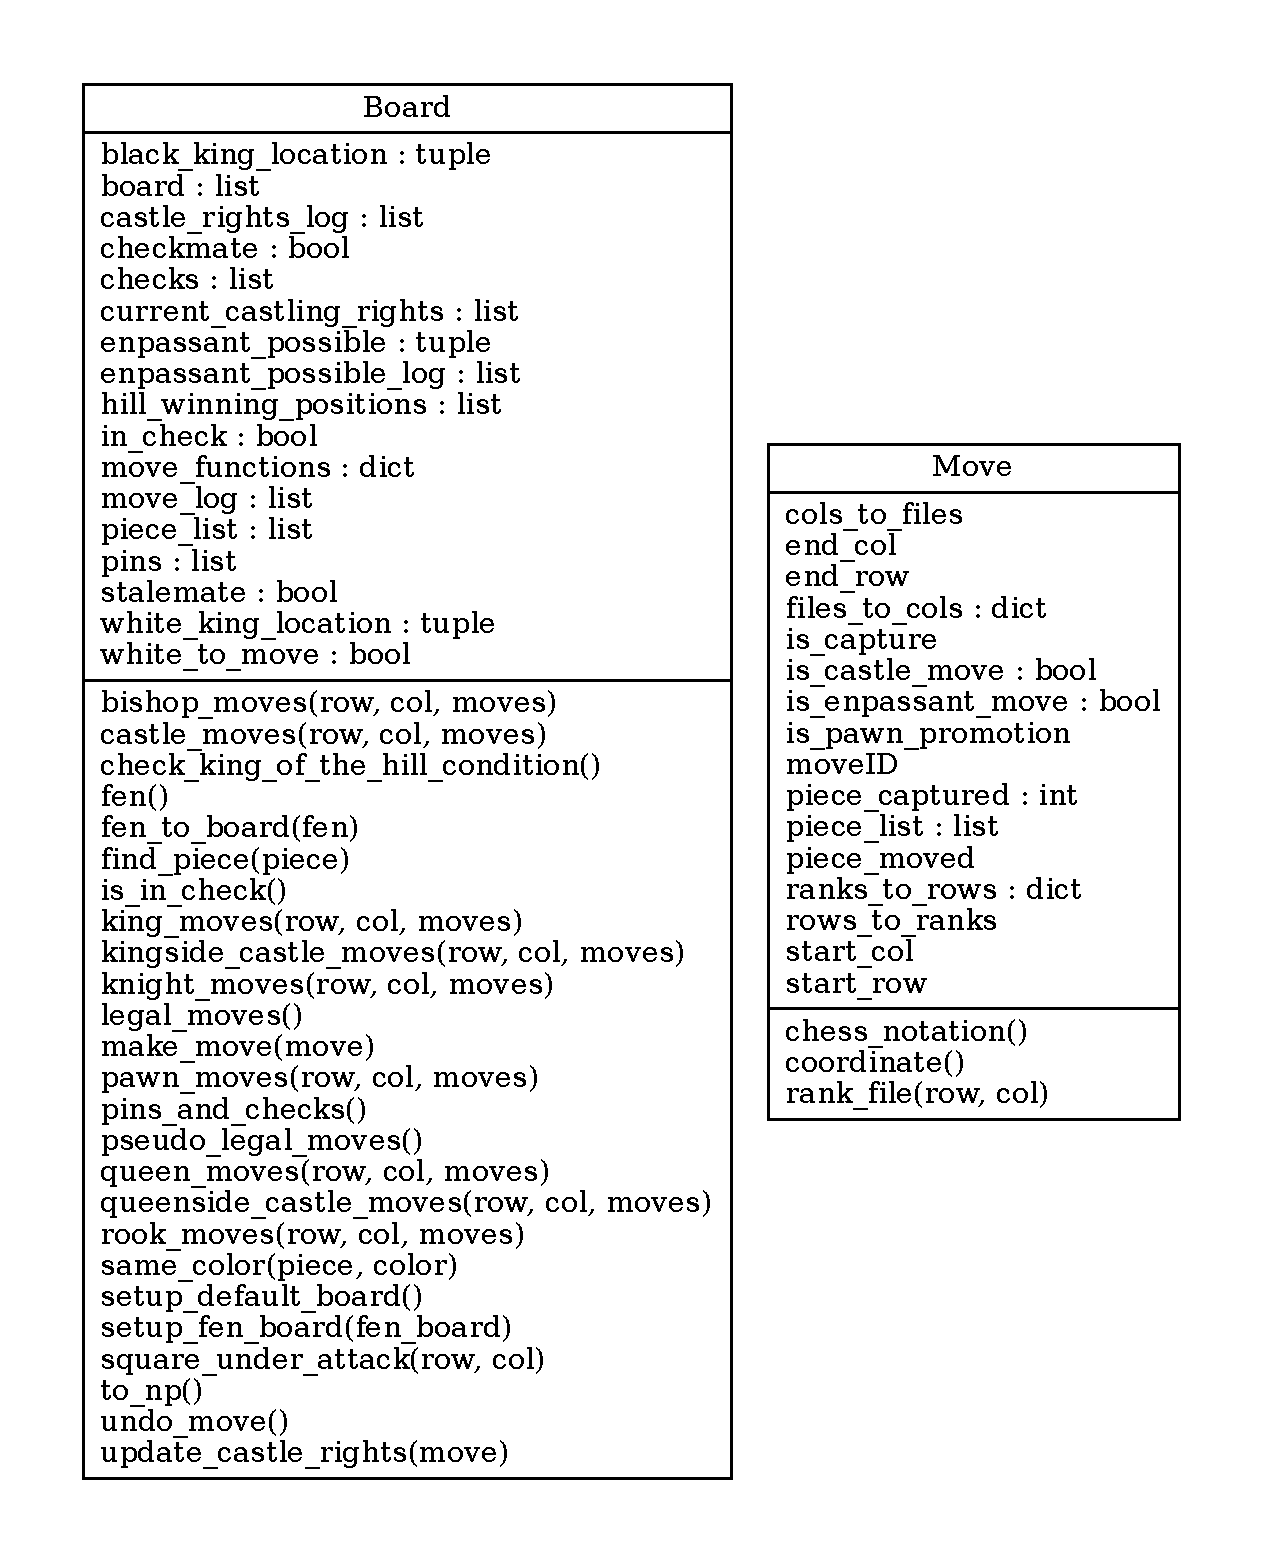
\includegraphics[width=0.7\linewidth, page=1]{reference/pics/class-diagram.pdf}
	\caption{Class diagram of the chess backend in its latest state}
  \label{fig:class-diagram}
\end{figure}

